\section{B-Tree}

\begin{tcolorbox}
	The implementations used for this task can be found \href{https://github.com/nngerncham/cs315_apal/tree/main/assignments/asn01/05-btree}{here}.
\end{tcolorbox}

\subsection{Optimal $b$}

In order to make the B-tree as fast as it can be, we want to minimize cache misses. This can be done by making sure that at least searches within the same node doesn't require extra load instructions. Thus, we want to be able to perfectly fit a node into a cache block for fast access.
In general, $b$ should be based on the size of the key-value pair when stored in memory especially if they could have a variety of sizes.
However, consider the case where both the key and the value are integers or \mintinline{c++}{int} for the sake of simplicity.
The size can then be interchanged for data types as well.
The amount of memory required for one key-value pair would be 64 bits or 8 bytes on a modern 64-bit machine.

Assume that the B-Tree is storing a pair of pointers for key and value and recall that a modern computer's cache line size is typically 32, 64, or 128 bytes. This means that we would be able to perfectly fit 4, 8, 16 pairs of keys and values into a single cache line for fastest access respectively. Therefore, the optimal value for $b$ would be either 4, 8, or 16 based on the these assumptions and the size of the cache line respectively.

\subsection{B-Tree vs. Ordered Map}

On the testing machine, the best performance comes from when $b = 18$ which is rather close to the estimate for the optimal $b$ when the cache line is 128 bytes from above. However, the performance is still very lacking compared to a built-in ordered map in C++ as the B-tree (with poor implementation) is approximately around \textit{7-12 times slower than the built-in ordered map}. (Maybe I just write bad code, which is pretty unfortunate.) Below are the results from the experiments.

\subsubsection{Results}

\subsubsection*{Insertion}

\begin{figure}[H]
	\begin{center}
		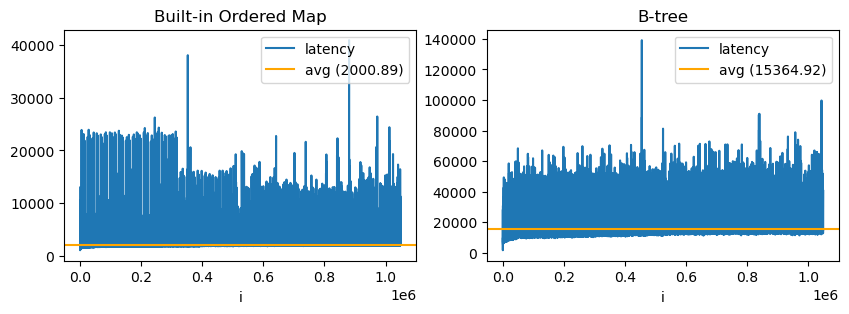
\includegraphics[width=0.9\textwidth]{05-insert-latencies.png}
		\caption{Insert latency of a C++ built-in ordered map and a B-tree}
		\label{fig:05-insert-latency}
	\end{center}
\end{figure}

\subsubsection*{Search}

\begin{figure}[H]
	\begin{center}
		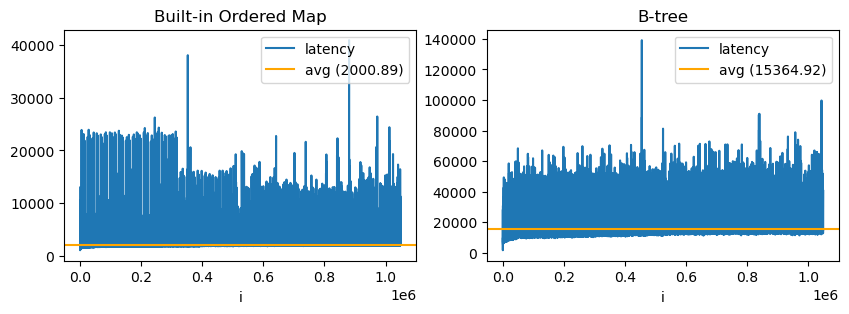
\includegraphics[width=0.9\textwidth]{05-insert-latencies.png}
		\caption{Search latency of a C++ built-in ordered map and a B-tree}
		\label{fig:05-search-latency}
	\end{center}
\end{figure}
